% 文档类(模板)
\documentclass[%
  type = bachelor,  % 本科论文(设计)
  % oneside,        % 单面模式
  twoside,          % 双面模式(openany)
]{nwafuthesis}
% 导言区

% 将需要载入的宏包统一在settings/package.tex中进行管理
% 请按自己的论文排版需求,加载需要的宏包

% TikZ绘图宏包
\usepackage{tikz}
% 卧图卧表宏包
\usepackage{lscape}
% 引号宏包
\usepackage{csquotes}
% 子图表宏包
\usepackage{subcaption}
% 双语标题宏包
\usepackage{bicaption}
% 合并表格行宏包
\usepackage{multirow}
% csv数据处理宏包
\usepackage{datatool}
% 单位符号宏包
\usepackage{siunitx}
% 跨页长表格宏包
\usepackage{longtable}
% 三线表宏包
\usepackage{booktabs}
% 新一代表格排版宏包
\usepackage{tabularray}
% 表格注释说明宏包
\usepackage{threeparttable}
% 带边框小页环境
\usepackage{boxedminipage2e}

%%% Local Variables:
%%% mode: latex
%%% TeX-master: "../main.tex"
%%% End:

% 将必要的设置统一在settings/format.tex中进行管理
% ==============LaTeX命令排版命令(排版示例文档时使用)========================
\newcommand\cs[1]{\texttt{\textbackslash#1}}
\newcommand\pkg[1]{\texttt{#1}\textsuperscript{PKG}}
\newcommand\env[1]{\texttt{#1}}
\newcommand{\note}[1]{{%
  \color{magenta}{\bfseries 注意:}\emph{#1}}}
%% ==================================================

% 设置插图目录
\graphicspath{{./figs/},{./logo/}}
%% ==================================================

% 引入tabularray的booktabs库
\UseTblrLibrary{booktabs}

%% 自定义相关的名称宏命令
%% ==================================================
% 西北农林科技大学各单位名称
\newcommand{\nwsuaf}{西北农林科技大学}
\newcommand{\cie}{信息工程学院}
\newcommand{\ca}{农学院}
\newcommand{\cpp}{植物保护学院}
\newcommand{\chc}{园艺学院}
\newcommand{\cast}{动物科技学院}
\newcommand{\cvm}{动物医学院}
\newcommand{\cf}{林学院}
\newcommand{\claa}{风景园林艺术学院}
\newcommand{\cnre}{资源环境学院}
\newcommand{\cwrae}{水利与建筑工程学院}
\newcommand{\cmee}{机械与电子工程学院}
\newcommand{\cfse}{食品科学与工程学院}
\newcommand{\celg}{葡萄酒学院}
\newcommand{\clsc}{生命科学学院}
\newcommand{\cst}{理学院}
\newcommand{\ccp}{化学与药学院}
\newcommand{\cem}{经济管理学院}
\newcommand{\cm}{马克思主义学院}
\newcommand{\chsd}{人文社会发展学院}
\newcommand{\dfl}{外语系}
\newcommand{\iec}{创新实验学院}
\newcommand{\ci}{国际学院}
\newcommand{\dpe}{体育部}
\newcommand{\cvae}{成人教育}
\newcommand{\iswc}{水土保持研究所}

%%% Local Variables:
%%% mode: latex
%%% TeX-master: "../main.tex"
%%% End:



% 编写测试文档用到的两个宏包,若不需要,可能删除
% 中文乱数假文宏包
\usepackage{zhlipsum}
% 最小工作示例(MWE)宏包,主要用于插图示例
\usepackage{mwe}
% 排版设置
\nwafuset{
% 论文格式
  style = {
    % font          = times*,           % 选择英文字体(需要安装有该字体,建议自动配置)
    % cjk-font      = adobe,            % 选择中文字体(需要安装有该字体,建议自动配置)
    hyperlink     = color,            % 超链接颜色
    % withchapter = false,            % 章标题是否为章模式(仅本科生需要)
    bib-resource  = {bib/thsis.bib}, % 参考文献数据源文件名,注意需要完整路径及后缀名
  },
% 信息录入
  info = {
    grade = {2022}, % 毕业年份(届)
    enroll = {2018}, % 入学年份(级)
    class-id = {2}, % 班级号
    btype = {paper}, % 本科类型(论文/设计)
    % btype = {design},
    title = { 基于GeoServer与OpenLayers的雨水资源GIS专题图设计与实现 }, % 中文题目
    title* = { Design and implementation of GIS thematic maps of rainwater resources based on GeoServer and OpenLayers}, % 英文题目
    department = { 信息工程学院 }, % 学院名称
    major = {计算机科学与技术}, % 专业
    author = { 高瑞 }, % 作者中文名称
    supervisor = { 孙红光 }, % 指导教师
    cosupervisor = {聂炎明}, % 协助指导教师
    date = {\datezh}, % 论文提交时间
    student-id = {2018012998}, % 学号
  },
}
% 录入摘要
\nwafuset{
  abstract = {
    abstractfile  = { contents/chap00-abs-zh.tex }, % 中文摘要文件名称,注意需要有.tex后缀名
    abstractfile* = { contents/chap00-abs-en.tex }, % 英文摘要文件名称,注意需要有.tex后缀名
    keywords      = {GIS, 雨水资源, 专题图,构建}, % 中文关键字列表,注意用英文逗号分隔。
    keywords*     = {GIS, rainwater resources, thematic maps, construction}, % 英文关键字列表,注意用英文逗号分隔
  },
}
% 正文区(有且只能有一个)
\begin{document}
% 这个命令用来关闭版心底部强制对齐,
% 可以减少不必要的 underfull \vbox 提示,但会影响排版效果
% \raggedbottom

% 由于论文模板中已设计了自动排版封面、摘要、目录等功能,
% 因此,无需手动排版。

% 主体部分是论文的核心
\mainmatter

% 建议采用多文件编译的方式编写论文,
% 比较好的做法是把每一章放进一个单独的 tex 文件里,
% 并在这里用 \include 导入,如:
% 本文件是示例论文的一部分
% 本文是论文的第一章:绪论
% 论文的主文件是位于上级目录的 `main.tex`

\chapter{绪论}

\section{研究背景和意义}

西北地区由陕西、甘肃、宁夏、青海、新疆和内蒙古6省(区)组成,地域辽阔,人口相对稀少,该区气候干旱,降水稀少,蒸发旺盛,这样特殊的地理位置及气候条件决定了西北地区水资源短缺,生态环境脆弱。该区光热资源和土地、矿产资源比较丰富,属于资源开发主导型地区。然而,西北地区的水资源问题是该地区当前及未来国民经济和社会发展的最大制约因素,已引起了国家和社会的广泛关注\cite{黄智煌邬娜-2}。

西北地区气候干旱、降雨稀少,全区多年平均降水量2300mm,而水面蒸发量高达1000~2600mm以上,是全国唯一降水量极度少于农田作物和天然植被需水量的地区。据资料分析,西北地区多年平均地表水资源量约为1463亿立方米,地下水资源量998亿立方米,地下水资源与地表水资源重复计算量789亿立方米,水资源总量1672亿立方米,人均水资源总量2189立方米,耕地亩均水资源量857立方米。从表面上看,内陆河流域的人均、亩均水资源量并不算少,但由于水资源与人口、耕地的地区分布极不均衡,有相当大一部分分布在地势高寒、自然条件较差的人烟稀少地区及无人区,而自然条件较好、人口稠密、经济发达的绿洲地区水资源量十分有限。黄河流域河川径流具有地区分布不均、年际变化大及连续枯水等特点,内陆河流域的水资源主要以冰雪融水补给为主,年内分配高度集中,汛期径流量可占全年径流量的80%,部分河流汛期陡涨,枯季断流,开发利用的难度较大。\cite{仇巍巍陈从喜-1}


GIS 本质是运行在计算机上的一种软件,其是一门综合性的学科,集成应用了地理学、地图学、计算机科学、遥感学等,构建成一个集数据采集、存储、分析、显示、管理、计算等为一体的地理信息系统。该系统基于计算机运行,对地理空间信息进行分析并处理成图,将地表现象和事物可视化的显示出来。从以上的分析可以看出,其强大的功能适用于水文水资源领域,像调查地下水资源、地表水资源状况,以及监测水质与江河湖泊的水位变化等。GIS 技术在水文水资源领域的良好运用,对于水资源管理和保护工作有着重要意义。\cite{张国治韩景琦-3}

“雨水资源监控管理系统”是结合气象站、墒情站、GIS地理系统等监测传感设备,对于天气、墒情、地表水资源(包括水库、蓄水池、河流、地面径流雨水)等数据进行实施监测与传输,结合计算机软件,对于区域性雨水资源情况和用水结构进行协同管理,辅助当地政府和企业单位充分利用与开发当地雨水资源。\cite{郭明华-4}

GIS雨水资源专题图便是将区域性水资源,天气、墒情、地表水资源(包括水库、蓄水池、河流、地面径流雨水)等信息可视化,便于农户政府企业等对雨水等资源进行合理管理与利用来缓解西北地区用水资源短缺等问题,这对于西北地区发展资源开发,提高经济增长率,改善人民生活等具有重大的现实意义。\cite{刘治华-5}


\section{研究现状}
\subsection{国内研究现状}

现在针对西北地区的水资源现状,主要采取了如下对策:第一,强化水资源开发利用与保护的规划和监督管理,严格实施建设项目审批和管理制度。一方面,要制定出合理的水资源开发与保护方面的规划与制度,另一方面,要加强管理人员执法能力、技术能力等能力培养,加强执法必要设备的配置;第二,加强水利基本建设,如建设必要的调水工程,将部分水资源从富裕地区调往贫水区,或将优质水调往劣质水区,以改善缺水地区或不良水质地区的生产生活环境,也为生态环境建设提供必要的支持;第三,建设现代化的高效节水型经济社会,如适当提高水价,尤其是工业行业的水价,减少对水的浪费。发展集雨节灌,以解决农村用水困难,补充城市生态环境用水;第四,坚决实施有计划地退耕还林、还草。而且在西部大开发战略中,也水土资源的合理开发和有效利用摆在了更加突出的位置,而实现雨水资源的有效利用是水资源开发的一个主要方式,但是现在有关科研单位和水利部门的实现探索,主要是如何将雨水资源保存下来,发展雨水集蓄利用等技术,以及如何合理的使用雨水资源等技术的研究,但是没有将各个地区的雨水资源分布,受天气土地等影响因素导致的雨水收集效率等通过系统的方式形成系统性的可供各用水单位参考的资料等。
而通过GIS专题图便可以很好地实现各个地区的雨水资源分布的可视化系统,使得用水单位对雨水资源的调配等方面有系统的参考。

\subsection{国外研究现状}
地理信息系统(GIS)是以计算机为基础的综合处理和空间数据分析系统,是集计算机科学、管理科学、信息科学、地学等为一体的新兴边缘研究领域。20世纪70年代,美国田纳西河流域管理局利用GIS技术处理分析各种流域数据,为流域管理和规划提供决策服务,GIS便开始逐渐应用于水文水资源领域。80年代后随着计算机技术的飞速发展,GIS与水文水资源领域也有了广泛结合。

在国外,Gupta等早在1977年就实现了将栅格型GIS数据管理工具用于流域规划。随后欧洲一些研究机构也联合开发了具有水文过程模拟、水污染控制、水资源规划等功能的流域规划决策支持系统“WATERWARE”。近年Carlo等在GIS平台上开发了Ag-PIE模型,用于评价由于农业生产造成的地表和地下水水质下降的程度。

自20世纪70年代美国田纳西河流域管理局利用GIS技术处理和分析各种流域数据,开始为流域管理提供决策服务以来,GIS技术亦广泛应用于国外的水资源管理中。如美国科罗拉多州的一些机构联合开发了科罗拉多河决策支持系统,GIS被用于流域空间的存储、检索、分析和显示,以便于科罗拉多河水资源的管理。在灌区的水资源管理方面,位于美国德克萨斯州Lower Rio Grande Valley的8个灌区较早地开发以GIS为基础的灌区管理系统(DMS)。

 在国外,Davis曾将HEC-1、HEC-2与 GIS结合对洪水、水质和土坡侵蚀进行了模拟,可很好地用于洪灾损失评估。
 
 在国外,为了支持各种层次的水资源和水环境管理,美国国家环保局基于GIS技术和地调局水文数据开发了全美河段文件。He等将AGNPS、GRASS与GRASS Water Works模型集成在一起,综合评价了非点源污染对美国密歇根州Cass河水质的影响,近年来,Boyle等建立的IDOR2D系统将水污染模型与GIS集成。
 
 国外的分布式水文模型起始于1969年,比较著名的有TOPMODEL、SHE、IHDM模型和美国农业部的SWAT模型,目前得到了长足发展并在多个地区进行了实践和应用。近年出现的基于不规则三角网格(TIN)构建出得完全分布式模型,只需原始栅格节点的5%~10%就可以充分描述流域地形的水文特征,大大提高了分布式模型的计算效率,为大型流域的水文模拟提供了可能,是今后分布式水文模型研究的热点。国内的分布式水文模型研究起步较晚,沈晓东等在研究降雨和下垫面自然地理参数空间分布的不均匀性对径流过程的影响基础上,提出一个动态分布式降雨径流流域模型,实现了基于栅格DEM的坡面产汇流与河道汇流的数值模拟;郭生练等建立了一个基于DEM的分布式流域水文物理模型,用来模拟小流域的降雨径流时空变化过程;任立良等考虑了流域空间的变异性,基于DEM建立了参考作物蒸散量的分布式模型;李兰等在提出的变动生态产流模式的概念基础上建立了LL-I分布式降雨径流模型,能明显改善模拟预报精度,适合不同水文特征地区的产汇流计算
\section{主要工作}

雨水资源GIS专题图整体架构主要设计工作如下:
%使用{\nwafuthesis}模板排版学位论文的工作流如\ref{fig:workflow}所示。
%
%\begin{figure}[!htb]
%  \centering
%  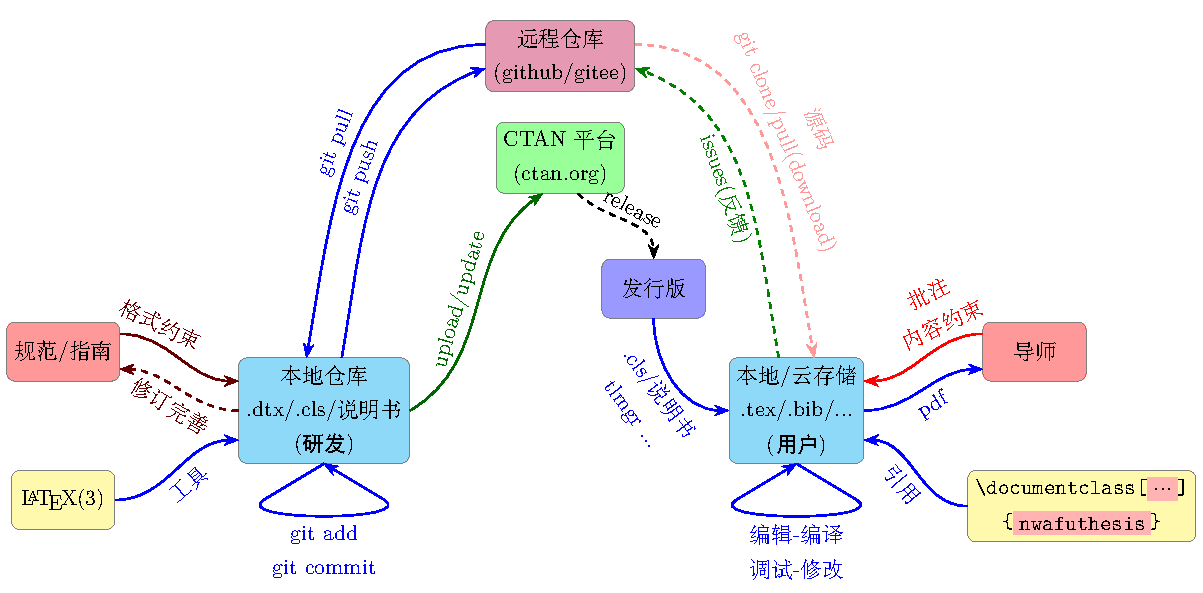
\includegraphics[width=0.85\textwidth]{figs/workflow}
%  \caption{模板工作流}
%  \label{fig:workflow}
%\end{figure}
\begin{enumerate}
	
\item 	数据设计:

GIS系统的数据按照性质的不同可以分为空间数据和属性数据,空间数据指地理空间对象的,属性数据包括地理空间对象的属性以及其他相关联的业务数据等。在了解GIS专题图在采集、存储、分析、研究、图示为一体的数据分析以及GIS专题图对于各种数据格式的定义等知识,GIS专题图的坐标系知识,为(历史、现在、未来)的水系信息,不同区域、时段等粒度的降雨信息,蒸散发信息,地下水信息,地形信息,不同区域粒度的土壤墒情,植被覆盖信息,光照、气温、降水信息,交通信息等为所需设计的雨水资源专题图设计合适的数据格式。
\item 	坐标系设计:

学习GIS专题图坐标系知识,结合系统需求分析以及与雨水资源各种元素因素特性,为雨水资源专题图中各种地形所需的不同的坐标系选择合适的坐标系。如图2所示。
\item	粒度设计

根据水资源不同元素因素的条件(历史、现在、未来)的水系信息,不同区域、时段等粒度的降雨信息,蒸散发信息,地下水信息,地形信息,不同区域粒度的土壤墒情,植被覆盖信息,光照、气温、降水信息等,设计不同时段区域类型等的粒度大小等信息。
\item	应用层设计

本系统的应用层主要是指IE,chrome,firhox等浏览器应用程序。本系统客户端设计采用“瘦客户端”的设计模式,即客户端无需安装任何插件即可进行地图的浏览、查询等操作,降低了对客户端配置的要求,减轻了客户端负担,用户只需普通IE等浏览器即可进行所有操作。本课题以AJAX技术为基础进行GIS专题图的开发,以XML作为与地图服务组件的数据传输协议。大大提升了系统的实用性和可扩展性等能力。
\item	基础底层设计

根据之前的坐标系设计,为不同坐标系下的数据信息设计各自的基础底层,例如地形信息需要基于海拔,地形3D信息的基础底层,而水资源分布只需基于平面的地图便可以表示。
\item 	影响因子设计

不同区域的水资源,如河流、水库、蓄水池、地下水、等水资源信息会受到各
种环境因素如,土壤类型,肥力,墒情,酸碱度,空气温湿度,分数,光照,
经纬度,海拔等因素影响,为了使得水资源信息更加准确,需要设计影响因子
作为水资源分布的参考要素。
\item 	操作图层设计

根据土壤墒情,植被覆盖信息,光照、气温、降水信息,地理信息等影响因子设计操作图层,使用户可以根据不同区域特定情况选择不同影响因子作用下的水资源分布,例如沙型土壤影响因子作用下的地下水的水资源较高,但是对于地表水资源便较少。

\item 	数据获取

采用ArcGIS Server服务,WMS(网络地图服务)、WFS(网络要素服务)等GIS数据服务以及ajax技术实现前后端数据通信,数据的获取。
\item 	数据可视化布局设计

使用OpenLayers和Pvechars库实现对应属性数据的可视化。编写代码实现研究内容中的各种GIS专题图,以及对GIS专题图和数据统计图进行整体组织和布局。
\end{enumerate}
\section{具体设计内容}

研究内容主要为雨水资源管理系统中的雨水资源GIS专题图的设计与实现。


1.	对水资源分布的历史、实时、未来等的信息按照不同的时段、区域、类型等粒度进行统计,并采用统计图(以及列表)的方式进行显示。


2.	水系信息的(历史、现在、未来)GIS专题图制作以及展示。

3.	不同区域、时段等粒度的降雨信息的(历史、现在、未来)GIS专题图制作以及展示。


4.	不同区域、时段、种植作物等粒度的蒸散发信息的(历史、现在、未来)GIS专题图制作以及展示。


5.	地下水信息的(历史、现在、未来)GIS专题图制作以及展示。


6.	地形信息的(历史、现在、未来)GIS专题图制作以及展示。

7.	不同区域粒度的土壤墒情之土壤类型、肥力、墒情、酸碱度等信息的(历史、现在、未来)GIS专题图制作以及展示。

8.	植被覆盖信息的(历史、现在、未来)GIS专题图制作以及展示。

9.	不同区域、时段等粒度的气候之光照、气温、降水等信息的(历史、现在、未来)GIS专题图制作以及展示。

10.	不同区域、时段等粒度的气候之光照、气温、降水等信息的(历史、现在、未来)GIS专题图制作以及展示。

11.	不同区域、时段等粒度的交通信息的GIS专题图制作以及展示。



\section{章节安排}
第一章和第二章主要是项目的主要设计内容,研究背景,研究现状以及实现技术等等,从第三章开始为项目的主体介绍,分为三章来介绍项目实现的成果,第三章主要是介绍本项目的需求分析,主要分为:功能需求,性能需求,界面需求,接口需求,第四章主要介绍雨水资源GIS专题图总体设计,主要为功能设计和数据库设计,第五章主要是介绍雨水资源专题图的详细设计与实现,主要为地表水系图,地下水系图,气候图。地表水系图分为河流水系图、蓄水池图、水库图、污水分布图等,地下水系图主要分为地下水分布图、土壤类型图、土壤含量图等,气候图则主要分为光照图、降雨图、温度图、风速风向图等。如\ref{fig:dirforest}所示。
\begin{figure}[!htb]%关于这些编译器的配置和使用,请参阅相关说明资料。
  \centering
  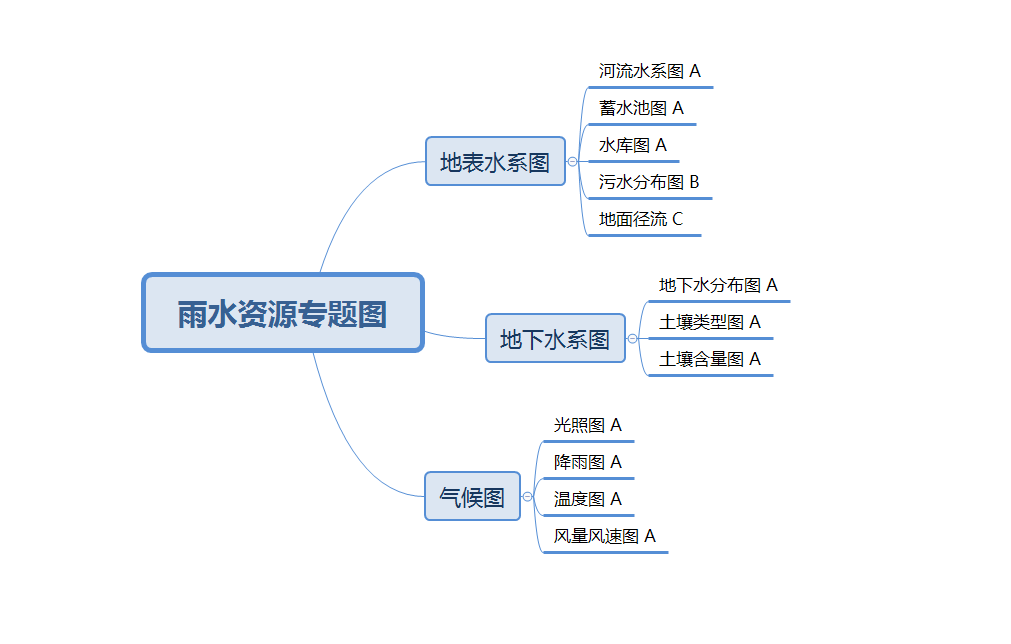
\includegraphics[width=0.60\textwidth]{figs/tree.png}
  \caption{雨水资源专题图分类}
  \label{fig:dirforest}
\end{figure}

%写作过程中的各个文件:
%

%完成部分或所有\verb|*.tex|撰写和修改后,可以在命令行使用 \verb|latexmk -xelatex main|
%进行编译输出\verb|main.pdf|文件,可以根据需要对结果\texttt{pdf}文件进行改名。
%
%也可以使用\texttt{TeXstudio}、\texttt{vscode}等GUI编辑器的进行编辑和编译输出。

%
%
%\note{}由于\nwafuthesis{}需要处理图、表、公式及参考文献等交叉引用,因此,
%往往需要多次编译才能得到正确的结果。为此,必须设置正确的编译方式和编译参数。
%关于多次编译的问题,大家可以浏览耿楠在B站发布的视频
%(\url{https://www.bilibili.com/video/BV1qa4y1v7my?spm_id_from=333.999.0.0})
%进行学习。



%如果论文需要双面打印的话,请务必修改文档类选项,编译双面打印用的 PDF 文件。
%具体地说,在主文件的头部,去除 \texttt{openany, oneside},
%改成 \texttt{twoside}。

%同时,建议注释\cs{nwafuset}命令中的\enquote{style/hyperlink = color},
%以\emph{取消超链接颜色}。

%%% Local Variables:
%%% mode: latex
%%% TeX-master: "../main.tex"
%%% End:

% 本文件是示例论文的一部分
% 本文件是论文的第二章:技术路线
% 论文的主文件位于上级目录的 `main.tex`

\chapter{实现技术介绍}



\section{GeoServer}
  GeoServer是开源项目,可以免费使用GeoServer,并具有自行修改、复制以及再分发的权利。同时,GeoServer还有 众多的优点:


\begin{enumerate}
 
   \item 用JAVA 语言编写、标准的J2EE架构、基于servlet 和 STRUTS 框架、支持高效的Spring 框架开发;
   \item 兼容WMS和WFS特性、支持WFS—T规范;
   \item 高级数据库支持PostGIS 、Shapefile、ArcSDE 、Oracle 、DB2、VPF 、MySQL、MapInfo 等;
   \item 支持上百种投影;
   \item 能够将网络地图输出为jpeg、gif、png、SVG、GML、KML 等格式;
   \item 能够运行在任何基于J2EE/Servle容器之上;
   \item 嵌入MapBuilder 支持AJAX 的地图客户端;
   \item 实现了在线编辑空间数据、生成专题地图;
   \item 地图发布是用xml 文件;
   \item 支持GOOGLE MAPS;
   \item 可发布KML 数据,与GoogleEarth 影像叠加,作出生动的应用;
\end{enumerate}



\section{Openlayers}
要想在浏览器中显示交互式的地图很难,因为浏览器默认的只是显示静态的图片,如PNG、JPEG等格式,要交互式很难,因为每一个点击和缩放,地图都要做出正确的反应。

OpenLayers 是一个专为Web GIS 客户端开发提供的JavaScript 类库包,主要是用于开发Web GIS客户端,用于实现标准格式发布的地图数据访问。从OpenLayers2.2版本以后,OpenLayers已经将所用到的Prototype.js组件整合到了自身当中,并不断在Prototype.js的基础上完善面向对象的开发,Rico用到地方不多,只是在OpenLayers.Popup.AnchoredBubble类中圆角化DIV。OpenLayers2.4版本以后提供了矢量画图功能,方便动态地展现“点、线和面”这样的地理数据。

OpenLayers支持Google Maps、Yahoo Map、微软Virtual Earth等资源,可以通过WMS服务调用其它服务器上的空间数据,通过WFS服务调用空间服务。在操作方面,OpenLayers 除了可以在浏览器中实现地图浏览的基本效果,如放大、缩小、平移等操作,进行选取面、选取线、要素选择、图层叠加等操作。

在操作方面,OpenLayers 除了可以在浏览器中帮助开发者实现地图浏览的基本效果,比如放大(Zoom In)、缩小(Zoom Out)、平移(Pan)等常用操作之外,还可以进行选取面、选取线、要素选择、图层叠加等不同的操作,甚至可以对已有的OpenLayers 操作和数据支持类型进行扩充,为其赋予更多的功能。例如,它可以为OpenLayers 添加网络处理服务WPS 的操作接口,从而利用已有的空间分析处理服务来对加载的地理空间数据进行计算。同时,在OpenLayers提供的类库当中,它还使用了类库Prototype.js 和Rico 中的部分组件,为地图浏览操作客户端增加Ajax 效果。

相对于另一个框架 OpenScales,OpenScales 是 OpenLayers 的 ActionScript 翻译,需要 FlashPlayer 支持才行,所以相比较来说,我们选择了原生的openlayers作为我们的实现技术。




%%% Local Variables: 
%%% mode: latex
%%% TeX-master: "../main.tex"
%%% End:

% 本文件是示例论文的一部分
%第三章 需求分析
% 论文的主文件位于上级目录的 `main.tex`
\chapter{雨水资源GIS专题图需求分析}



\section{专题图总体概述}

GIS专题地图是以普通地图为地理基础,着重表示制图区域内某一种或几种自然要素或社会经济现象的地图。

专题地图的内容主要由两部分构成:专题内容和地理基础,前者为地图上突出表示的自然要素或社会经济现象及其有关特征;后者为用以表明专题图要素空间位置与地理背景的普通地图内容。

这类地图的显示特点是,作为该图主题的专题图内容予以详尽表示,其地理基础内容则视主题而异,有选择地表示某些相关要素。

因此我们通过对具体问题进行具体分析,分析得到本项目的具体需求,以便设计出专题更加鲜明,符合各个要求需求的GIS专题图。

\subsection{系统属性}

该系统是雨水资源监控管理系统的一个子系统,用于将指定区域的水资源种类情况以及水资源分布情况以GIS专题图形式展示给用户,能够让用户更清晰、直观的看到其所关心的部分,方便用户更好的协调各个区域的水资源调用实现水资源的高效利用。

\subsection{开发背景}

开发目的是为了方便用户查看水资源的收集、分布等情况,通过GIS专题图形式为用户提供可视化方便理解的信息,为水资源的调度提供决策支持,应用的目标是使该系统的操作人员以及该系统覆盖地区下的所有居民、政府人员等可以直观地了解各个地区的水资源储量等信息。

\subsection{功能概述}

主要功能为以GIS专题图的形式展示土壤类型、肥力、墒情、酸碱度等信息;展示空气温湿度、风速风向、光照等信息;展示各个地区所属的地下水、水库、河流等水量信息;一起后信息和植被覆盖信息等为参考,展示各个地区的蒸散发信息。

\subsection{用户特点}

主要使用人员为相关工作人员、技术人员、政府人员、企业人员以及定边县的居民等。
其中相关工作人员、技术人员、政府人员、企业人员具备相关技能知识培训且有使用过类似的系统的操作经验,对于本系统可以很快上手使用,而对于普通居民用户需要进行必要的操作培训才能灵活使用该系统。


%对于数学公式的排版在\enquote{lshort-zh-cn.pdf}的第四章给出了基本的使用方法,
%请大家阅读学习。其内容对大多数人来说已经足够用了,但是如果不能解决问题的话
%建议大家求助于搜索引擎或者有经验的人,这也不失为一个好办法。
%
%常见的几个学习\LaTeX{}数学公式排版的资源链接如下:
%
%\begin{itemize}
%  \item 数学排版常见问题集:
%        \url{https://www.latexstudio.net/index/details/index/mid/635}
%  \item \pkg{amsmath}手册中译:
%        \url{https://www.latexstudio.net/index/details/index/mid/706}
%  \item \LaTeX{}公式备忘单:
%        \url{https://www.latexstudio.net/index/details/index/mid/1052.html}
%\end{itemize}

\section{具体需求}

\subsection{功能需求}

\begin{enumerate}
	\item 土壤信息:
	
	以GIS专题图的形式展示土壤类型、肥力、墒情酸碱度等信息,不同地区的土壤类型用不同颜色表示,肥力墒情和酸碱度信息通过用户点击来显示出某个地区的肥力墒情酸碱度信息。
    \item 气候信息:
 
    以GIS专题图的形式展示气候信息,主要为空气温湿度,风速风向,光照等信息,在特定区域地图为底图,以图标的形式展示风向和光照信息,不同颜色展示温度信息,当点击各种图标时,会显示出风向,光照强度,具体温湿度信息。
    \item 降雨信息:
    
    以GIS专题图的形式展示各个区域的降雨信息,包括过去、现在、未来等情况。
    \item 蓄水信息:
    使用GIS专题图来展示各个区域的河流水库地下水的蓄水情况,不同地下水储量情况可以使用不同颜色来表示,水库在地图上使用原点标识出来,河流可采用点击各个区域出现具体数据来展示。
    \item{蒸散发信息}
    
    通过对气候信息和植被覆盖信息的处理来得出各个区域的蒸散发强度信息,采用不同颜色或者蒸发动态图标展示。不同区域有蒸散发具体数据。
    
\end{enumerate}

\subsection{性能需求}

\begin{enumerate}
	\item{可靠性}
	
	要求系统能经受时效和压力测试,系统平台具备不少于100个访问并发的能力。
	
	\item{效率}
	
	对展示界面要求简洁明了,符合用户的观看习惯,GIS专题图的显示要快速直观。
	
	\item{安全性}
	
	高安全性,能够防止网站数据被非法篡改。
	
	\item{可维护性}
	
	方案和系统的架构须紧密跟踪主流技术标准,开放性好,便于系统的升级维护、以及与各种信息系统进行集成。
\end{enumerate}


\subsection{界面需求}

界面需简洁明了,符合用户观看习惯,采用数据大屏的形式展示GIS专题图,并且根据需求可在专题图周围添加数据图表以便更加方便观察各种数据。

\subsection{接口需求}

本项目主要是展示相关地区的地理,雨水资源,气候等信息,所以对于接口来说主要是为主动从后端获取信息,因此通过webservice进行前后端通信,选择json数据进行数据的传输。





%%% Local Variables: 
%%% mode: latex
%%% TeX-master: "../main.tex"
%%% End:

% 本文件是示例论文的一部分
%第四章 总体设计
% 论文的主文件位于上级目录的 `main.tex`
\chapter{雨水资源GIS专题图总体设计}
\section{设计思路}
\begin{enumerate}
	\item 具体问题具体分析,获取精准需求。
	
	GIS专题图具有地图内容主题化的特点,因此具体的需求必须精准化才能使得GIS专题图的设计更好的贴合项目,更好的使用户查看,使用,理解。例如,对于降雨信息而言,我们必须抓住降雨的主要特点:降雨量,可利用降雨量,总降雨量,降雨量范围等。以此来精准获得GIS专题图应该展示的内容,对于次要要素选择其他方式进行展示。
	\item GIS专题图分类
	
	随着GIS技术的日益成熟,作为地理分析结果重要表现形式的专题地图,也在不断发展、创新和应用,现在已经衍生出了GIS专题图的具体分类,比如:独立值专题图,点密度专题图,范围专题图,等级符号专题图,时序专题图,多比例尺专题图,多变量专题图等,因此参考具体需求选取具体种类的专题图十分必要。
	\item 专题图功能设计
	
	除了专题图具体展示的内容以外,还需要考虑其他粒度的展示功能,比如时序功能,例如降雨信息,我们需要考虑过去一段时间内的降雨信息的展示等。所以需要进行专题图的功能设计,让专题图展示的内容更加完善。
	\item 界面设计
	
	当设计好专题图需要展示的内容时,接下来我们就需要如何设计界面,让专题图在大屏上展示出来,具体功能bottom键的放置位置等,以及次要要素的展示设计等。
\end{enumerate}

\section{功能设计}
由需求设计具体功能。
\subsection{功能描述}
%土壤信息
土壤信息功能设计如(\ref{1})所示:

    \begin{table}[H]
	\centering
	\caption[土壤信息]{土壤信息功能描述及流程}
	\label{1}
	\begin{tabular}{|c|c|c|c|}
		
		\hline
		功能编号&01&功能名称&土壤信息\\
		\hline
		\multicolumn{2}{|c|}{功能描述}&\multicolumn{2}{c|}{\multirow{1}{0.7\textwidth}{以GIS专题图的形式展示土壤类型、肥力、墒情酸碱度等信息,不同地区的土壤类型用不同颜色表示,肥力墒情和酸碱度信息通过用户点击来显示出某个地区的肥力墒情酸碱度信息。}}\\[6ex]
		\hline
		\multicolumn{2}{|c|}{功能流程}&\multicolumn{2}{c|}{\multirow{1}{0.7\textwidth}{当用户点击首页时,界面会加载指定地图,以不同颜色区分出各个地区不同的土壤类型情况,当用户放置在(或点击)某个区域时,会显示出此地区的肥力墒情和酸碱度信息,此专题图为静态地图,只有当影响土壤类型肥力墒情和酸碱度信息的出现时,信息才会进行更新。}}\\[10ex]
		\hline
		

	\end{tabular}
    \end{table}
%气候信息
气候信息功能设计如(\ref{2})所示:

\begin{table}[H]
	\centering
	\caption[气候信息]{气候信息功能描述及流程}
	\label{2}
	\begin{tabular}{|c|c|c|c|}
		
		\hline
		功能编号&02&功能名称&气候信息\\
		\hline
		\multicolumn{2}{|c|}{功能描述}&\multicolumn{2}{c|}{\multirow{1}{0.7\textwidth}{以GIS专题图的形式展示气候信息,主要为空气温湿度,风速风向,光照等信息,在定边县地图为底图,以图标的形式展示风向和光照信息,不同颜色展示温度信息,当点击各种图标时,会显示出风向,光照强度,具体温湿度信息。}}\\[10ex]
		\hline
		\multicolumn{2}{|c|}{功能流程}&\multicolumn{2}{c|}{\multirow{1}{0.7\textwidth}{用户点击气候信息时,会展示出定边县与气候相关的GIS专题图,用户会在各个区域粒度的风向标,光照标识以及不同区域不同颜色的温湿度情况,当用于放置在(或点击)某个标识或者区域时,会具体展示出光照强度、风速数据以及具体的温湿度数据。此专题图为动态地图,会随时随着当时当地的气候变化来变化信息数据,(可设置不同时间粒度变化的次数来满足用户需求,地图类型可参考天气预报形式)}}\\[16ex]
		\hline
		
		
	\end{tabular}
\end{table}
%降雨信息
降雨信息功能设计如(\ref{3})所示:

\begin{table}[H]
	\centering
	\caption[降雨信息]{降雨信息功能描述及流程}
	\label{3}
	\begin{tabular}{|c|c|c|c|}
		
		\hline
		功能编号&01&功能名称&降雨信息\\
		\hline
		\multicolumn{2}{|c|}{功能描述}&\multicolumn{2}{c|}{\multirow{1}{0.7\textwidth}{以GIS专题图的形式展示各个区域的降雨信息,包括过去、现在、未来等情况}}\\[4ex]
		\hline
		\multicolumn{2}{|c|}{功能流程}&\multicolumn{2}{c|}{\multirow{1}{0.7\textwidth}{用户点击降雨信息时,会展示当前也就是现在的降雨情况,使用白色到蓝色覆盖区域来展示现在的降雨大小情况,当用户放置(或点击)某个区域时会展示具体降雨量信息,降雨信息点击还包括选择日期,分为过去以及未来预测的降雨情况,展示情况和现在情况一样,过去以及未来的天数根据数据库以及天气预报具体情况来设计。此地图也应为动态地图,但是由于降雨特殊情况可以将时间粒度放宽一些。}}\\[16ex]
		\hline
		
		
	\end{tabular}
\end{table}
%蓄水信息
蓄水信息功能设计如(\ref{4})所示:

\begin{table}[H]
	\centering
	\caption[蓄水信息]{蓄水信息功能描述及流程}
	\label{4}
	\begin{tabular}{|c|c|c|c|}
		
		\hline
		功能编号&01&功能名称&蓄水信息\\
		\hline
		\multicolumn{2}{|c|}{功能描述}&\multicolumn{2}{c|}{\multirow{1}{0.7\textwidth}{使用GIS专题图来展示各个区域的河流水库地下水的蓄水情况,不同地下水储量情况可以使用不同颜色来表示,水库在地图上使用原点标识出来,河流可采用点击各个区域出现具体数据来展示}}\\[10ex]
		\hline
		\multicolumn{2}{|c|}{功能流程}&\multicolumn{2}{c|}{\multirow{1}{0.7\textwidth}{当用户点击蓄水信息时,会展示当前的各个区域的蓄水情况,不同区域会看到不同的颜色,这代表了不同区域地下水储量的不同,还会看到一些圆点,这些代表了各个地区的水库位置,当放置(或点击)圆点时会展示出水库的具体信息(名称,蓄水量等),当放置(或点击)具体区域时会展示流经该地区的河流具体信息(河流名称,具体流量等),此为静态地图,当出现用水情况时,GIS专题图信息才会改变。}}\\[16ex]
		\hline
		
		
	\end{tabular}
\end{table}
蒸散发信息
蒸散发信息功能设计如(\ref{5})所示:

\begin{table}[H]
	\centering
	\caption[蒸散发信息]{蒸散发信息功能描述及流程}
	\label{5}
	\begin{tabular}{|c|c|c|c|}
		
		\hline
		功能编号&01&功能名称&蒸散发信息\\
		\hline
		\multicolumn{2}{|c|}{功能描述}&\multicolumn{2}{c|}{\multirow{1}{0.7\textwidth}{通过对气候信息和植被覆盖信息的处理来得出各个区域的蒸散发强度信息,采用不同颜色或者蒸发动态图标展示。不同区域有蒸散发具体数据。}}\\[6ex]
		\hline
		\multicolumn{2}{|c|}{功能流程}&\multicolumn{2}{c|}{\multirow{1}{0.7\textwidth}{当用户点击蒸散发信息时,会展示出不同区域不同蒸散发直观信息,当放置(或点击)具体区域时,会展示出具体区域的蒸散发信息数据。由于气候信息为动态信息,所以蒸散发信息也为动态信息,随时变化。}}\\[8ex]
		\hline
		
		
	\end{tabular}
\end{table}




\subsection{功能视图}

\section{数据库设计}

\subsection{河流数据库设计}

\begin{table}[H]
	\centering
	\caption[河流数据]{河流数据库表}
	\begin{tabular}{cccccc}
		\toprule
		名            & 类型      & 长度 &是否可为null & 键 & 注释\\
		\midrule
		id            & varchar  & 100  & 否 & 是 & 河流数据id \\
		riv\_name     & varchar  & 255  &是  & 否 & 河流名称   \\
		riv\_qua      & varchar  & 255  &是  & 否 & 河流水质   \\
		riv\_change   & float    & 255  &是  & 否 & 河流变化量 \\
		riv\_flow     & float    & 255  &是  & 否 & 河流流量   \\
		riv\_ev       & float    & 255  & 是 & 否 & 蒸发量     \\
		detail\_id    & varchar  & 100  & 是 & 否 & 河流详情id \\
		create\_time  & datatime &      &是  & 否 & 创建时间   \\
		delete\_time  &datatime  &      & 是 & 否 & 删除时间   \\ 
		\bottomrule
	\end{tabular}
\end{table}
\subsection{蓄水池数据库设计}

\begin{table}[H]
	\centering
	\caption[蓄水池数据]{蓄水池数据库表}
	\begin{tabular}{cccccc}
		\toprule
		名            & 类型      & 长度 &是否可为null & 键 & 注释\\
		\midrule
		id            & varchar  & 100  & 否 & 是 & 蓄水池数据id \\
		imp\_name     & varchar  & 255  &是  & 否 & 蓄水池名称   \\
		imp\_qul      & varchar  & 255  &是  & 否 & 蓄水池水质   \\
		imp\_change   & float    & 255  &是  & 否 & 蓄水池变化量 \\
		riv\_total    & float    & 255  &是  & 否 & 蓄水池储存总量   \\
		riv\_ev       & float    & 255  & 是 & 否 & 蒸发量     \\
		detail\_id    & varchar  & 100  & 是 & 否 & 蓄水池详情id \\
		create\_time  & datatime &      &是  & 否 & 创建时间   \\
		delete\_time  &datatime  &      & 是 & 否 & 删除时间   \\ 
		\bottomrule
	\end{tabular}
\end{table}
\subsection{水库数据库设计}
\begin{table}[H]
	\centering
	\caption[水库数据]{水库数据库表}
	\begin{tabular}{cccccc}
		\toprule
		名            & 类型      & 长度 &是否可为null & 键 & 注释\\
		\midrule
		id            & varchar  & 100  & 否 & 是 & 水库数据id \\
		re\_name      & varchar  & 255  &是  & 否 & 水库名称   \\
		re\_qual      & varchar  & 255  &是  & 否 & 水库水质   \\
		re\_change    & float    & 255  &是  & 否 & 水库水变化量 \\
		re\_total     & float    & 255  &是  & 否 & 水库储存总量   \\
		re\_ev        & float    & 255  & 是 & 否 & 蒸发量     \\
		detail\_id    & varchar  & 100  & 是 & 否 & 水库详情id \\
		create\_time  & datatime &      &是  & 否 & 创建时间   \\
		delete\_time  &datatime  &      & 是 & 否 & 删除时间   \\ 
		\bottomrule
	\end{tabular}
\end{table}
\subsection{污水数据库设计}
\begin{table}[H]
	\centering
	\caption[污水数据]{污水数据库表}
	\begin{tabular}{cccccc}
		\toprule
		名            & 类型      & 长度 &是否可为null & 键 & 注释\\
		\midrule
		id            & varchar  & 100  & 否 & 是 & 污水id \\
		se\_change     & varchar  & 255  &是  & 否 & 污水变化量   \\
		se\_total      & varchar  & 255  &是  & 否 & 污水储存总量   \\
		se\_locate   & float    & 255  &是  & 否 & 地理位置 \\
		se\_metal    & float    & 255  &是  & 否 & 金属含量   \\
		se\_amni       & float    & 255  & 是 & 否 & 氨氮含量     \\
		se\_oxy    & varchar  & 255  & 是 & 否 & 溶解氧含量 \\
		se\_origin&varchar & 255 &是 & 否&产生来源\\
		create\_time  & datatime &      &是  & 否 & 创建时间   \\
		delete\_time  &datatime  &      & 是 & 否 & 删除时间   \\ 
		\bottomrule
	\end{tabular}
\end{table}
\subsection{地下水数据库设计}
\begin{table}[H]
	\centering
	\caption[地下水数据]{地下水数据库表}
	\begin{tabular}{cccccc}
		\toprule
		名            & 类型      & 长度 &是否可为null & 键 & 注释\\
		\midrule
		id            & varchar  & 100  & 否 & 是 & 地下水数据id \\
		uw\_qul     & varchar  & 255  &是  & 否 & 地下水水质   \\
		uw\_change      & varchar  & 255  &是  & 否 & 地下水变化量   \\
		uw\_total   & float    & 255  &是  & 否 & 地下水储存总量 \\
		uw\_ev       & float    & 255  & 是 & 否 & 蒸发量     \\
		detail\_id    & varchar  & 100  & 是 & 否 & 地下水详情id \\
		create\_time  & datatime &      &是  & 否 & 创建时间   \\
		delete\_time  &datatime  &      & 是 & 否 & 删除时间   \\ 
		\bottomrule
	\end{tabular}
\end{table}
\subsection{土壤数据库设计}
\begin{table}[H]
	\centering
	\caption[土壤数据]{土壤数据库表}
	\begin{tabular}{cccccc}
		\toprule
		名            & 类型      & 长度 &是否可为null & 键 & 注释\\
		\midrule
		id           & varchar  & 100  & 否 & 是 & 土壤id \\
		so\_type     & varchar  & 255  &是  & 否 & 土壤类型   \\
		so\_wat      & float    & 255  &是  & 否 & 水分   \\
		so\_so       & float    & 255  & 是 & 否 & 盐分     \\
        so\_humidity & float    & 255  & 是 & 否 & 湿度     \\
        so\_fertility & float    & 255  & 是 & 否 & 肥力     \\
        so\_n       & float    & 255  & 是 & 否 & 含氮量     \\
        so\_locate  & float    & 255  & 是 & 否 & 位置     \\
		create\_time  & datatime &      &是  & 否 & 创建时间   \\
		delete\_time  &datatime  &      & 是 & 否 & 删除时间   \\ 
		\bottomrule
	\end{tabular}
\end{table}

\subsection{光照数据库设计}
\begin{table}[H]
	\centering
	\caption[光照数据]{光照数据库表}
	\begin{tabular}{cccccc}
		\toprule
		名            & 类型      & 长度 &是否可为null & 键 & 注释\\
		\midrule
		id            & varchar  & 100  & 否 & 是 & 光照id \\
		ill\_big     & varchar  & 255  &是  & 否 & 光照强度   \\
		ill\_thre      & varchar  & 255  &是  & 否 & 阙值   \\
		ill\_val   & float    & 255  &是  & 否 & 光合有效辐射 \\
		ill\_total     & float    & 255  &是  & 否 & 总辐射量   \\
		ill\_locate       & varchar    & 255  & 是 & 否 & 地理位置     \\
		create\_time  & datatime &      &是  & 否 & 创建时间   \\
		delete\_time  &datatime  &      & 是 & 否 & 删除时间   \\ 
		\bottomrule
	\end{tabular}
\end{table}

\subsection{降雨数据库设计}
\begin{table}[H]
	\centering
	\caption[降雨数据]{降雨数据库表}
	\begin{tabular}{cccccc}
		\toprule
		名            & 类型      & 长度 &是否可为null & 键 & 注释\\
		\midrule
		id            & varchar  & 100  & 否 & 是 & 气候降雨id \\
		wa\_de     & varchar  & 255  &是  & 否 & 露点   \\
		wa\_val      & varchar  & 255  &是  & 否 & 有效降雨量   \\
		wa\_total   & float    & 255  &是  & 否 & 总雨量 \\
	    wa\_thre     & float    & 255  &是  & 否 & 阙值   \\
		wa\_locate   & varchar    & 255  & 是 & 否 & 地理位置     \\
		create\_time  & datatime &      &是  & 否 & 创建时间   \\
		delete\_time  &datatime  &      & 是 & 否 & 删除时间   \\ 
		\bottomrule
	\end{tabular}
\end{table}

\subsection{温度数据库设计}
\begin{table}[H]
	\centering
	\caption[温度数据]{温度数据库表}
	\begin{tabular}{cccccc}
		\toprule
		名            & 类型      & 长度 &是否可为null & 键 & 注释\\
		\midrule
		id            & varchar  & 100  & 否 & 是 & 温度id \\
		tem\_tem     & varchar  & 255  &是  & 否 & 温度   \\
		tem\_thre\_tem      & varchar  & 255  &是  & 否 & 阙值   \\
		tem\_dew   & float    & 255  &是  & 否 & 湿度 \\
		tem\_thre\_dew     & float    & 255  &是  & 否 & 阙值   \\
		tem\_locate   & varchar    & 255  & 是 & 否 & 地理位置     \\
		create\_time  & datatime &      &是  & 否 & 创建时间   \\
		delete\_time  &datatime  &      & 是 & 否 & 删除时间   \\ 
		\bottomrule
	\end{tabular}
\end{table}

\subsection{风数据库设计}
\begin{table}[H]
	\centering
	\caption[风数据]{风数据库表}
	\begin{tabular}{cccccc}
		\toprule
		名            & 类型      & 长度 &是否可为null & 键 & 注释\\
		\midrule
		id            & varchar  & 100  & 否 & 是 & 风id \\
		wid\_spe      & varchar  & 255  &是  & 否 & 风速   \\
		wid\_thre      & varchar  & 255  &是  & 否 & 阙值   \\
		wid\_direction   & float    & 255  &是  & 否 & 风向 \\
		wa\_locate   & varchar    & 255  & 是 & 否 & 地理位置     \\
		create\_time  & datatime &      &是  & 否 & 创建时间   \\
		delete\_time  &datatime  &      & 是 & 否 & 删除时间   \\ 
		\bottomrule
	\end{tabular}
\end{table}

%%% Local Variables: 
%%% mode: latex
%%% TeX-master: "../main.tex"
%%% End:

% 本文件是示例论文的一部分
% 论文的主文件位于上级目录的 `main.tex`

\chapter{雨水资源GIS专题图详细设计与实现}

\section{功能设计}

\subsection{模块设计}
通过需求分析总体设计分析之后,将GIS专题图项目分为四个模块,主要为:大屏左面数据栏,右边数据栏,GIS专题图,头部导航栏四个模块,通过将数据展示栏和专题图还有导航栏分模块,可以使后期进行系统迭代更加方便,也符合模块化开发的标准和要求,主要模块分类如\ref{fig:module}所示:

\begin{figure}[!htb]%关于这些编译器的配置和使用,请参阅相关说明资料。
	\centering
	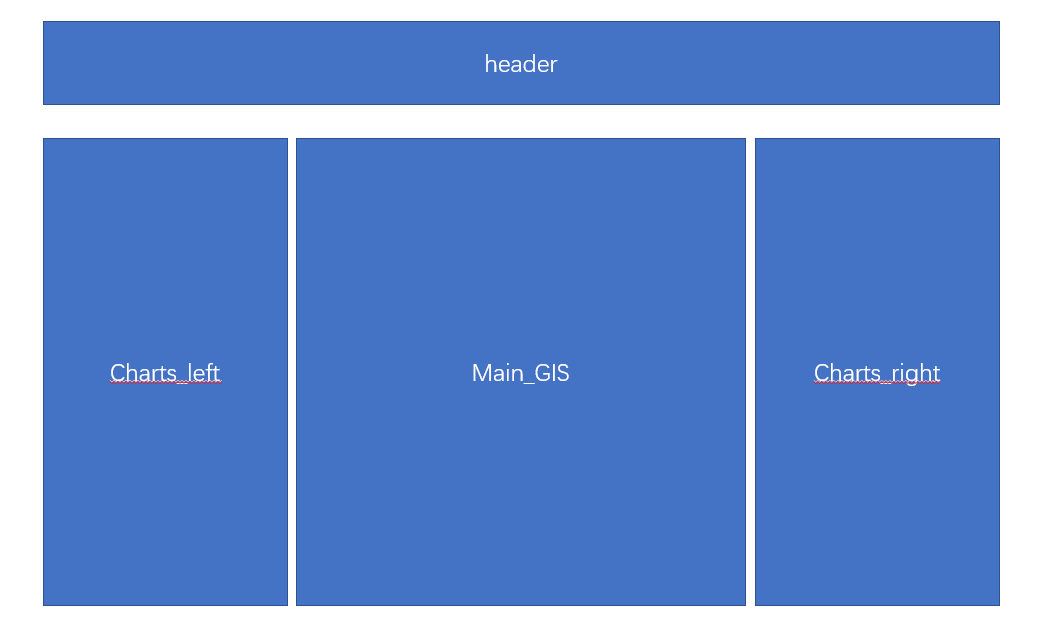
\includegraphics[width=0.60\textwidth]{figs/main.png}
	\caption{模块布局分类}
	\label{fig:module}
\end{figure}

\subsection{界面设计}


\section{地表水系设计}

\subsection{河流专题图设计}
\subsection{蓄水池专题图设计}
\subsection{水库专题图设计}
\section{地下水系设计}
\subsection{地下水分布专题图}
\subsection{土壤含量图}
\subsection{土壤类型图}
\section{气候图}
\subsection{光照专题图}
\subsection{降雨专题图}
\subsection{风速风向专题图}


%%% Local Variables: 
%%% mode: latex
%%% TeX-master: "../main.tex"
%%% End:

% 本文件是示例论文的一部分
% 论文的主文件位于上级目录的 `main.tex`

\chapter{结论与展望}

结个论,展个望。

\section{结果}
用\LaTeX 写论文还是蛮轻松的。

\section{展望}
以后还要设计更多,更方便的命令来实现高效\LaTeX 论文撰写。



%%% Local Variables: 
%%% mode: latex
%%% TeX-master: "../main.tex"
%%% End:

%
% 打印参考文献列表
%\addbibresource[location=local]{bib/sample.bib}

\bibmatter*
\printbibliography[heading=bibintoc]
%\addbibresource[location=local]{bib/thsis.bib}
% 排版附录,可选
\appendix
% 本文件是示例论文的一部分
% 论文的主文件位于上级目录的 `main.tex`

\chapter{查重和其他注意事项}

\section{查重}

先说结论:{\large\enquote{知网完全支持pdf查重}},学校学院也接收pdf格式的论文,这个无需担心。

如果导师只接受Word版论文,那也就没有办法了,你就用Word吧,只要下点功夫,也不是个事。建议大家提前和指导老师进行沟通,以确认能不能提交pdf格式论文。

\section{批注}
在论文撰写过程中,pdf格式的论文,批注是一个问题,如果对\LaTeX 和基于Git的版本管理并不了解,就只能使用Adobe Acrobat、平板手写等软件,对pdf文件本身进行批注,相比于word确实有些麻烦。

强烈推荐使用Git\footnote{\url{https://git-scm.com/}}、Beyond Compare\footnote{\url{https://www.scootersoftware.com/}}等工具,辅以\LaTeX 本身的注释进行批注以及版本管理,非常清晰直观,操作也简单。

\section{毕业设计与毕业论文的区别}
这里特别对使用本模板的本科同学们做出提醒,请查看毕业设计基本信息中的毕设类别,共有两类:\enquote{毕业设计}和\enquote{毕业论文}。因此在\verb!\documentclass[]{nwafuthesis}!的选项中需要标明\textbf{Design}(毕业设计)或者\textbf{Paper}(毕业论文),使论文使用正确的封面和独创性声明。

\section{单面打印\& 双面打印}
学校并没有规定论文打印的方式,考虑到部分同学有双面打印的需求,可以在文档选项中使用oneside/twoside来切换单面打印和双面打印。

\section{封面打印\& 装订}
建议大家去指定打印部门打印封面并装订,以免打印装订不合格。

\section{批注}
在论文撰写过程中,pdf格式的论文,批注是一个问题,如果对\LaTeX 和基于Git的版本管理并不了解,就只能使用Adobe Acrobat、平板手写等软件,对pdf文件本身进行批注,相比于word确实有些麻烦。

强烈推荐使用Git\footnote{\url{https://git-scm.com/}}、Beyond Compare\footnote{\url{https://www.scootersoftware.com/}}等工具,辅以\LaTeX 本身的注释进行批注以及版本管理,非常清晰直观,操作也简单。

\section{毕业设计与毕业论文的区别}
这里特别对使用本模板的本科同学们做出提醒,请查看毕业设计基本信息中的毕设类别,共有两类:\enquote{毕业设计}和\enquote{毕业论文}。因此在\verb!\documentclass[]{nwafuthesis}!的选项中需要标明\textbf{Design}(毕业设计)或者\textbf{Paper}(毕业论文),使论文使用正确的封面和独创性声明。

\section{单面打印\& 双面打印}
学校并没有规定论文打印的方式,考虑到部分同学有双面打印的需求,可以在文档选项中使用oneside/twoside来切换单面打印和双面打印。

\section{封面打印\& 装订}
建议大家去指定打印部门打印封面并装订,以免打印装订不合格。

\section{批注}
在论文撰写过程中,pdf格式的论文,批注是一个问题,如果对\LaTeX 和基于Git的版本管理并不了解,就只能使用Adobe Acrobat、平板手写等软件,对pdf文件本身进行批注,相比于word确实有些麻烦。

强烈推荐使用Git\footnote{\url{https://git-scm.com/}}、Beyond Compare\footnote{\url{https://www.scootersoftware.com/}}等工具,辅以\LaTeX 本身的注释进行批注以及版本管理,非常清晰直观,操作也简单。

\section{毕业设计与毕业论文的区别}
这里特别对使用本模板的本科同学们做出提醒,请查看毕业设计基本信息中的毕设类别,共有两类:\enquote{毕业设计}和\enquote{毕业论文}。因此在\verb!\documentclass[]{nwafuthesis}!的选项中需要标明\textbf{Design}(毕业设计)或者\textbf{Paper}(毕业论文),使论文使用正确的封面和独创性声明。

\section{单面打印\& 双面打印}
学校并没有规定论文打印的方式,考虑到部分同学有双面打印的需求,可以在文档选项中使用oneside/twoside来切换单面打印和双面打印。

\section{封面打印\& 装订}
建议大家去指定打印部门打印封面并装订,以免打印装订不合格。

\section{批注}
在论文撰写过程中,pdf格式的论文,批注是一个问题,如果对\LaTeX 和基于Git的版本管理并不了解,就只能使用Adobe Acrobat、平板手写等软件,对pdf文件本身进行批注,相比于word确实有些麻烦。

强烈推荐使用Git\footnote{\url{https://git-scm.com/}}、Beyond Compare\footnote{\url{https://www.scootersoftware.com/}}等工具,辅以\LaTeX 本身的注释进行批注以及版本管理,非常清晰直观,操作也简单。

\section{毕业设计与毕业论文的区别}
这里特别对使用本模板的本科同学们做出提醒,请查看毕业设计基本信息中的毕设类别,共有两类:\enquote{毕业设计}和\enquote{毕业论文}。因此在\verb!\documentclass[]{nwafuthesis}!的选项中需要标明\textbf{Design}(毕业设计)或者\textbf{Paper}(毕业论文),使论文使用正确的封面和独创性声明。

\section{单面打印\& 双面打印}
学校并没有规定论文打印的方式,考虑到部分同学有双面打印的需求,可以在文档选项中使用oneside/twoside来切换单面打印和双面打印。

\section{封面打印\& 装订}
建议大家去指定打印部门打印封面并装订,以免打印装订不合格。

\section{批注}
在论文撰写过程中,pdf格式的论文,批注是一个问题,如果对\LaTeX 和基于Git的版本管理并不了解,就只能使用Adobe Acrobat、平板手写等软件,对pdf文件本身进行批注,相比于word确实有些麻烦。

强烈推荐使用Git\footnote{\url{https://git-scm.com/}}、Beyond Compare\footnote{\url{https://www.scootersoftware.com/}}等工具,辅以\LaTeX 本身的注释进行批注以及版本管理,非常清晰直观,操作也简单。

\section{毕业设计与毕业论文的区别}
这里特别对使用本模板的本科同学们做出提醒,请查看毕业设计基本信息中的毕设类别,共有两类:\enquote{毕业设计}和\enquote{毕业论文}。因此在\verb!\documentclass[]{nwafuthesis}!的选项中需要标明\textbf{Design}(毕业设计)或者\textbf{Paper}(毕业论文),使论文使用正确的封面和独创性声明。

\section{单面打印\& 双面打印}
学校并没有规定论文打印的方式,考虑到部分同学有双面打印的需求,可以在文档选项中使用oneside/twoside来切换单面打印和双面打印。

\section{封面打印\& 装订}
建议大家去指定打印部门打印封面并装订,以免打印装订不合格。

\section{附录的图表}

附录中的图表:

\begin{figure}[htb]
  \centering
  
\includegraphics[width=3cm]{nwafu-circle}
  \caption{一个校徽}
\end{figure}


\begin{table}[htb]
  \centering
  \caption[城市人口]{城市人口数量排名 (source: Wikipedia)}
  \begin{tabular}{lr}
    \toprule
    城市 & 人口 \\
    \midrule
    Mexico City & 20,116,842\\
    Shanghai & 19,210,000\\
    Peking & 15,796,450\\
    Istanbul & 14,160,467\\
    \bottomrule
  \end{tabular}
\end{table}

\section{附录中的公式}

附录中的公式:

\begin{align}
d(\mathbf{p},\mathbf{q}) = d(\mathbf{q},\mathbf{p}) & = \sqrt{(q_1-p_1)^2 + (q_2-p_2)^2 + \cdots + (q_n-p_n)^2} \\
& = \sqrt{\sum_{i=1}^n (q_i-p_i)^2}
\end{align}

\chapter{后记}

\section{吐槽}

\verb!\begin{轻松+愉快}!

做模板过程中遇到的大问题,在于如何正确理解学校对论文格式的要求。
虽然有《本科毕业设计(论文)撰写格式要求》、《研究生学位论文撰写要求》,
但这些要求依然不够细致,因为那些要求都是假定你用 Word 来写论文的,要求里的内容是 Word 设置的操作方法,
所以还要先学习 Word 的排版算法,因此,本模板
但还有很多细节部分,因为能力有限,没能实现。

\verb!\end{愉快+轻松}!

\section{明天}

转眼间n年过去,又到了写毕业论文的时候了,一直想完成我们学校的毕业论文\LaTeX{}模板,今天总算有了一个初稿。

目前, \nwafuthesis{} 应该还有相当多的问题,但没有用户的话,由于作者能力有限,很难发现这些问题,
还请各位使用 \nwafuthesis{} 的先行者们(Pioneers) 能及时反馈意见和建议。

愿所有使用 \nwafuthesis{} 的人,不会被评审老师指责格式问题。

\section{吐槽}

\verb!\begin{轻松+愉快}!

做模板过程中遇到的大问题,在于如何正确理解学校对论文格式的要求。
虽然有《本科毕业设计(论文)撰写格式要求》、《研究生学位论文撰写要求》,
但这些要求依然不够细致,因为那些要求都是假定你用 Word 来写论文的,要求里的内容是 Word 设置的操作方法,
所以还要先学习 Word 的排版算法,因此,本模板
但还有很多细节部分,因为能力有限,没能实现。

\verb!\end{愉快+轻松}!

\section{明天}

转眼间n年过去,又到了写毕业论文的时候了,一直想完成我们学校的毕业论文\LaTeX{}模板,今天总算有了一个初稿。

目前, \nwafuthesis{} 应该还有相当多的问题,但没有用户的话,由于作者能力有限,很难发现这些问题,
还请各位使用 \nwafuthesis{} 的先行者们(Pioneers) 能及时反馈意见和建议。

愿所有使用 \nwafuthesis{} 的人,不会被评审老师指责格式问题。

\section{吐槽}

\verb!\begin{轻松+愉快}!

做模板过程中遇到的大问题,在于如何正确理解学校对论文格式的要求。
虽然有《本科毕业设计(论文)撰写格式要求》、《研究生学位论文撰写要求》,
但这些要求依然不够细致,因为那些要求都是假定你用 Word 来写论文的,要求里的内容是 Word 设置的操作方法,
所以还要先学习 Word 的排版算法,因此,本模板
但还有很多细节部分,因为能力有限,没能实现。

\verb!\end{愉快+轻松}!

\section{明天}

转眼间n年过去,又到了写毕业论文的时候了,一直想完成我们学校的毕业论文\LaTeX{}模板,今天总算有了一个初稿。

目前, \nwafuthesis{} 应该还有相当多的问题,但没有用户的话,由于作者能力有限,很难发现这些问题,
还请各位使用 \nwafuthesis{} 的先行者们(Pioneers) 能及时反馈意见和建议。

愿所有使用 \nwafuthesis{} 的人,不会被评审老师指责格式问题。

\section{吐槽}

\verb!\begin{轻松+愉快}!

做模板过程中遇到的大问题,在于如何正确理解学校对论文格式的要求。
虽然有《本科毕业设计(论文)撰写格式要求》、《研究生学位论文撰写要求》,
但这些要求依然不够细致,因为那些要求都是假定你用 Word 来写论文的,要求里的内容是 Word 设置的操作方法,
所以还要先学习 Word 的排版算法,因此,本模板
但还有很多细节部分,因为能力有限,没能实现。

\verb!\end{愉快+轻松}!

\section{明天}

转眼间n年过去,又到了写毕业论文的时候了,一直想完成我们学校的毕业论文\LaTeX{}模板,今天总算有了一个初稿。

目前, \nwafuthesis{} 应该还有相当多的问题,但没有用户的话,由于作者能力有限,很难发现这些问题,
还请各位使用 \nwafuthesis{} 的先行者们(Pioneers) 能及时反馈意见和建议。

愿所有使用 \nwafuthesis{} 的人,不会被评审老师指责格式问题。

\section{吐槽}

\verb!\begin{轻松+愉快}!

做模板过程中遇到的大问题,在于如何正确理解学校对论文格式的要求。
虽然有《本科毕业设计(论文)撰写格式要求》、《研究生学位论文撰写要求》,
但这些要求依然不够细致,因为那些要求都是假定你用 Word 来写论文的,要求里的内容是 Word 设置的操作方法,
所以还要先学习 Word 的排版算法,因此,本模板
但还有很多细节部分,因为能力有限,没能实现。
\verb!\end{愉快+轻松}!

\section{明天}

转眼间n年过去,又到了写毕业论文的时候了,一直想完成我们学校的毕业论文\LaTeX{}模板,今天总算有了一个初稿。

目前, \nwafuthesis{} 应该还有相当多的问题,但没有用户的话,由于作者能力有限,很难发现这些问题,
还请各位使用 \nwafuthesis{} 的先行者们(Pioneers) 能及时反馈意见和建议。

愿所有使用 \nwafuthesis{} 的人,不会被评审老师指责格式问题。




% 排版致谢
\backmatter
% 致谢
% 如果使用声明扫描页,将可选参数指定为扫描后的 PDF 文件名,例如:
% \begin{acknowledgement}[scan-statement.pdf]
\begin{acknowledgement}

研究生的生活即将结束,在这期间收获了很多,有过喜悦,有过成功,有过失败,
也有过迷茫,总之成长了许多。很庆幸也很荣幸得到了这么多人的支持和帮助。在此
向一直以来指导我的老师、关心我的亲友致以诚挚的感谢。

首先,感谢我的博士导师XXX研究员、XXX研究员的悉心指导,
二位老师渊博的知识、严谨的治学态度、对科学问题敏锐的洞察力和敬业的工作精神
对我有着潜移默化的影响,是我毕生学习的榜样。
在论文撰写过程中,二位老师从选题、试验指导和论文修改等方面都给予了许多指导。
师恩难表,纵使心中怀有万般感激之情,却皆非千万言语所能表达。
再次向恩师XXX老师、XXX老师、XXX老师致以诚挚的谢意,感谢您们的辛勤付出,
祝愿恩师阖家欢乐,身体健康,工作顺利。

感谢XXX教授、XXX研究员、 XXX研究员、 XXX研究员和XXX研究员
等开题指导老师对我的开题报告给予的客观评价与宝贵意见。 
感谢XXX教授、  XXX研究员、XX教授和XXX研究员
在学位答辩中提出的宝贵意见和建议。

感谢XX副研究员、XXX副教授,XX教授,XXX研究员等在论文思路、
修改和试验等工作中给予的指点和帮助。感谢XXX老师、XXX高工
从我研究生入学伊始便给予的极大帮助与关怀,二位老师为人处世方式
和认真负责的工作态度深刻地影响着我。

感谢XXXXXXXXX大学XXX博士、XXX博士和XXX博士等在合作工作中开展给予的大力支持与帮助。

感谢在学习和生活中帮助过我的同学,
感谢XXX、XXX、XXX和XXX等同学们对我的指导和照顾,
感谢XXX、XXX,XXX、XXX和XXX等同学们对我的帮助。
感谢XXX的同伴们在生活中和学习上给予的关心和帮助。

感谢我的家人,感谢我的父亲、母亲、岳父、岳母,
在我仿徨和无助的时候给予的鼓励、支持和理解,
以及学习和生活无微不至的照顾与关怀,是您们默默付出让我能更好地完成我的学业,
祝福您们身体健康,工作顺利, 万事如意。

特别感谢我挚爱的妻子XXX女士对于我学习工作的无私支持;
执汝手,共同行,莫问风疏雨聚,此后余生,与卿相伴。

感谢西北农林科技大学XXX重点实验室、研究生院和教学发展中心等
为我提供的良好学习环境和试验条件。

特别鸣谢信息工程学院耿楠教授团队开发的\nwafuthesis{}学位论文
\LaTeX{}模板,该模板为我节约了大量的论文编排时间,使我能够
专注于论文内容的思考与组织。同时,在论文写作过程中耿楠教授在\LaTeX{}
技术方面给予的全面指导与支持。

最后,感谢所有关心和帮助过我的人。也向所有的答辩评审委员致以真诚的谢意!\\

\begin{flushright}
         XXX

二〇二一年六月于\quad 杨凌
\end{flushright}

\newpage

我走了很远的路,吃了很多的苦,才将这份博士学位论文送到你的面前。二十二载求学路,一路风雨泥泞,许多不容易。如梦一场,仿佛昨天一家人才团聚过。

出生在一个小山坳里,母亲在我十二岁时离家。父亲在家的日子不多,即便在我病得不能自己去医院的时候,也仅是留下勉強够治病的钱后又走了。我十七岁时,他因交通事故离世后,我哭得稀里糊涂,因为再得重病时没有谁来管我了。同年,和我住在一起的婆婆病放,真的无能为力。她照顾我十七年,下葬时却仅是一副薄薄的棺材。另一个家庭成员是老狗小花,为父亲和婆婆守过坟,后因我进城上高中而命不知何时何处所终。如兄长般的计算机启蒙老师邱浩没能看到我的大学录取通知书,对我照顾有加的师母也在不惑之前匆匆离开人世。每次回去看他们,这一座座坟茔都提示着生命的每一分钟都弥足珍贵。

人情冷暖,生离死别,固然让人痛苦与无奈,而贫穷则可能让人失去希望。家徒四壁,在煤油灯下写作业或者读书都是晚上最开心的事。如果下雨,保留节目就是用竹笋壳塞瓦缝防漏雨。高中之前的主要经济来源是夜里抓黄鳞、周末钓鱼、养小猪崽和出租水牛,那些年里,方圆十公里的水田和小河都被我用脚测量过无数次。被狗和蛇追,半夜落水,因蓄电瓶进水而摸黑逃回家中;学费没交,黄鳝却被父亲偷卖了,然后买了肉和酒,都是难以避免的事。

人后的苦尚且还能克服,人前的尊严却无比脆弱。上课的时候,因拖欠学费而经常被老师叫出教室约谈。雨天湿漉着上课,屁股后面说不定还是泥。夏天光着脚走在滚烫的路上。冬天穿着破旧衣服打着寒颤穿过那条长长的过道领作业本。这些都可能成为压垮骆驼的最后一根稻草。如果不是考试后常能从主席台领奖金,顺便能贴一墙奖状满足最后的虚荣心,我可能早已放弃。

身处命运的漩涡,耗尽心力去争取那些可能本就是稀松平常的东西,每次转折都显得那么的身不由己。幸运的是,命运到底还有一丝怜惜。进入高中后,学校免了全部学杂费,胡叔叔一家帮助解决了生活费。进入大学后,计算机终于成了我一生的事业与希望,胃溃疡和胃出血也终与我作别。

从家出发坐大巴需要两个半小时才能到县城,一直盼着走出大山。从矩光乡小学、大寅镇中学、仪陇县中学、绵阳市南山中学,到重庆的西南大学,再到中科院自动化所,我也记不清有多少次因为现实的压力而觉得自己快扛不下去了。这一路,信念很简单,把书念下去,然后走出去,不枉活一世。世事难料,未来注定还会面对更为复杂的局面。但因为有了这些点点滴滴,我已经有勇气和耐心面对任何困难和挑战。理想不伟大,只愿年过半百,归来仍是少年,希望还有机会重新认识这个世界,不辜负这一生吃过的苦。最后如果还能做出点让别人生活更美好的事,那这辈子就赚了。

\vfill
\begin{flushright}
  中科院博士\  黄国平
\end{flushright}
\vfill


\newpage

子在川上曰,逝者如斯夫,不舍昼夜。自吾去蜀入秦,凡五年矣。昔之来者,翩翩素衣,白马银鞍,谈笑无忌。今将去也,堪堪而立,褐面黄须,肱股生腴。不得少瑜之梦笔,唯学祖狄而闻鸡。心高气傲以格钛二铝铌之物,智短才疏稍致材料加工之知。为此浅陋之文,以资博士之谋,诚不胜惶恐也。

初入长安,即为恩师所知遇,幸何如之。恩师曾公,名讳上卫下东,少有才名。师夷西学,以涉重洋,修诸德国,而报故邦。求索未知,惟日孜孜,正襟治学,不尝稍忘。及至聘为教授,时年仅三十有四耳。潜心于经典,焚膏以继晷。学问博如四海,非唯囿于简牍。每亲临工厂,必鱼贯相请,凡所问者莫不相答。尝有经年不解之惑,观之如庖丁之牛,解之以经理,人皆称善,莫不拜服。吾师声名之隆者如此。自吾拜于门下,言传之,身教之,伏九不怠。及其斧正拙笔,字斟之,句酌之,晨昏弗懈。为学莫重于尊师,恩师循循以导,谆谆而教,恩德未可胜计,无论尽报。

予以二八之年求学于外,背井辗转已逾十年矣。进不得衣锦还乡,以光门庭,退未尝趋庭鲤对,而事双亲。其为子也,殊不孝也。人之行,莫大于孝。夫致孝者,怀橘卧冰,温衾恣蚊。无报严君之德,何如三迁之恩。吾素远游无方,岁末而归,十数日复去。独见故乡十年无夏,不察父母容颜渐改。父母年逾天命,两鬓霜凝,尤以垂垂之姿,而为版筑之作。每念及斯,愧也,疚也,恨无地也。吾弟求学于成都,学业既成,此诚不胜之喜也。幼时尾从终日,及长而别,少聚多离。愚兄痴长五岁,孝悌两违,贤弟勿见责也。

学贵得师,亦贵得友。朋曰共砚,友曰志同。承蒙见遇,铭诸五内。清风明月同唱苏子,高山流水共操五音。刀笔可录春秋,缣帛难表衷言。敬列诸君之名于文末,以表谢忱,倘有阙漏,唯乞见谅耳。

  感谢 \LaTeX 和 \nwafuthesis,帮我节省了不少时间。

\vfill
\begin{flushright}
  西北工业大学博士\  郑友平
\end{flushright}
\vfill

\newpage


东北大学信息科学与工程学院自动化专业2017届毕业生米威名花了三天的时间写了这篇致谢。致谢里,他感谢了母校和师长无微不至的关心与爱护以及母亲含辛茹苦的照顾。米威名现已保研清华大学自动化系。
先来欣赏一下理工科大神的文言文致谢吧!

致谢:

公元二千一七年,岁次丁酉,初夏之月,威名拙论乃告杀青。理微辞穷,未敢称凌云之作,镂心鸟迹,得不效相如之叹?于是凭窗啜饮,寄情遐思。

忆余初入东大,未及弱冠,书生意气,挥斥方遒,或废寝以搜读先哲,或忘食而亲验知行。浮云朝露,过隙白驹,距吾始书尔来已春秋有四,于今毕业,年齿已趋而立。户牅之外,万物滋荣,熙来攘往,景致阙如昨日;堂室之内,漫展书卷,激昂文字,然威名早已有苍颜白发矣。

文凭两纸霜鬓两行,黄粱一枕功名一场,此皆书生寻常,乏善可陈。然威名身蒙寸草春晖之恩情,春风化雨之陶冶,润物无声之教化,育诲之恩,重胜泰山,虽衔环结草不能报之万一。是以情造文,铭而致谢。

威名古襄平人氏,布衣世家,聿修祖德,孝悌累洽。襁褓之时,家徒四壁,父苦工在外,母荆钗持家,亏得亲邻接济方得度日,后父以技长,渐为小康。髫龀入蒙,受教庠序,趋庭鲤对,每日不辍。时吾腹诗三百,音字无差。本就天伦,然世无常,父猝而远去,唯留母子相濡。此近十载,吾母吐哺无稍息,咽苦不颦眉。蓼蓼者莪,匪莪伊蒿,欲报之德,昊天罔极!

及吾稍长,志求门楣光耀以报顾复,于是负笈求学,欢会长乖。闻道远行,慈母手线,怜儿夜寒。子在关山外,慈母念他乡。孔子曰,立身行道,以显父母;《诗经》云,夙兴夜寐,无忝尔所生。何有于威名哉!此威名胡跪而叩谢者一也。

吾校东大,国之成均。肇于九一八国难之将近,辗转十四载抗战之狼烟。溯源沈水,奄宅奉天。临清朝陪都宫殿之前庭,接民国张氏帅府之后坊。苍松掩路,翠柏当庭。宁图晨钟,央园月朗。俊彦迭代,济济一堂。自强不息以树帜,知行合一以闻章。

威名不才,三尺微命。薄德寡智,有辱斯文。母校慈垂,翼我缥囊。沐浴清化,问学课堂。克明畯德,知止后安。吾尝于宁恩承内,望书卷万轴,乃知科学之堂奥,人文之博深。吾尝于何世礼中,聆名家讲学,方觉大师之风范,匠心之精运。吾亦尝漫行于五五,听夜雨梧桐,泠泠作响,感四时寒暑之潜移,觉宇宙天地之苍凉,哀人生往来于须臾,叹砺志奋发以图强。母校恩养,没齿难忘。此威名胡跪而叩谢者二也。

余自入东大以来,累受师长教育之恩。恩师张先生云洲,温恭和蔼,德才兼具。于威名之所学,吾师循循善诱,发蒙启蔽,苦心孤诣,鱼渔双授;于威名之修身,吾师以身作则,行端表正,不言之教,桃下之蹊。吾辈性骄,常拒管教,师亦不弃嫌,呕心沥血,方有余今日之成。余心感念,早已视之如父。

而于本论文之撰写,自题目选定至文献查阅,自实验设计至机理探撷,自纲路结构至文段末节,皆得吾师贾子熙,导师张涛悉心指点,谢无尽焉。此间感科研之路漫漫,志当上下而求索。亦再恩导师张涛不厌吾愚,允余北面承贽,以沐清华之泽,承先辈弦歌,勉夙愿之怀,此桃李之恩,片纸难详。《诗》曰:赫赫师尹,民具尔瞻。歌曰:云山苍苍,江水泱泱。先生之风,山高水长。艟艨巨舰,非桨舵导引之助不能乘风破浪;北溟鲲鹏,非长风托举之力不能垂翼九天。此威名胡跪而叩谢者三也。

诚惶诚恐,飏拜稽首。

\vfill
\begin{flushright}
  东北大学信息科学与工程学院\  米威名
\end{flushright}
\vfill




\end{acknowledgement}


% 个人简历, 本科生可选
\begin{resume}

  xxxx 年 xx 月 xx 日出生于 xx 省 xx 县。

  xxxx 年 9 月考入 xx 大学 xx 系 xx 专业,xxxx 年 7 月本科毕业并获得 xx 学士学位。

  xxxx 年 9 月免试进入 xx 大学 xx 系攻读 xx 学位至今。

  \researchitem[发表的学术论文] % 发表的和录用的合在一起

  \begin{publications}
    \item Yang Y, Ren T L, Zhang L T, et al. Miniature microphone with silicon-
      based ferroelectric thin films. Integrated Ferroelectrics, 2003,
      52:229-235. (SCI 收录, 检索号:758FZ.)
    \item 杨轶, 张宁欣, 任天令, 等. 硅基铁电微声学器件中薄膜残余应力的研究. 中国机
      械工程, 2005, 16(14):1289-1291. (EI 收录, 检索号:0534931 2907.)
    \item 杨轶, 张宁欣, 任天令, 等. 集成铁电器件中的关键工艺研究. 仪器仪表学报,
      2003, 24(S4):192-193. (EI 源刊.)
    \item Yang Y, Ren T L, Zhu Y P, et al. PMUTs for handwriting recognition. In
      press. (已被 Integrated Ferroelectrics 录用. SCI 源刊.)
    \item Wu X M, Yang Y, Cai J, et al. Measurements of ferroelectric MEMS
      microphones. Integrated Ferroelectrics, 2005, 69:417-429. (SCI 收录, 检索号
      :896KM)
    \item 贾泽, 杨轶, 陈兢, 等. 用于压电和电容微麦克风的体硅腐蚀相关研究. 压电与声
      光, 2006, 28(1):117-119. (EI 收录, 检索号:06129773469)
    \item 伍晓明, 杨轶, 张宁欣, 等. 基于MEMS技术的集成铁电硅微麦克风. 中国集成电路,
      2003, 53:59-61.
  \end{publications}

  \researchitem[发表专利] % 有就写,没有就删除
  \begin{achievements}
    \item 任天令, 杨轶, 朱一平, 等. 硅基铁电微声学传感器畴极化区域控制和电极连接的
      方法: 中国, CN1602118A. (中国专利公开号)
    \item Ren T L, Yang Y, Zhu Y P, et al. Piezoelectric micro acoustic sensor
      based on ferroelectric materials: USA, No.11/215, 102. (美国发明专利申请号)
  \end{achievements}

\end{resume}



\end{document}
